% Toolbar icon: reload from disk — the classic two-arc refresh glyph.
%
% Deliberately NOT the same drawing as `reset` (which is a single near-full
% circular arrow, used for "reset camera"): two half-arcs chasing each other
% read as "re-read the file", and having the two actions share one glyph would
% be misleading in a menu that offers both.
\documentclass[tikz,border=2mm]{standalone}
\usetikzlibrary{arrows.meta,calc}
\begin{document}
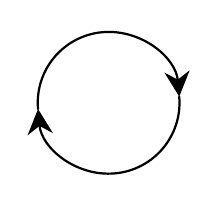
\begin{tikzpicture}[line width=1.3pt, line cap=round, line join=round, >=Stealth, x=1mm,y=1mm]
  % Upper arc, sweeping clockwise, arrowhead at the right.
  \draw[thick, -{Stealth[length=3.2mm,width=3.2mm]}] (185:9) arc (185:5:9);
  % Lower arc, sweeping back, arrowhead at the left.
  \draw[thick, -{Stealth[length=3.2mm,width=3.2mm]}] (5:9) arc (5:-175:9);
\end{tikzpicture}
\end{document}
